\documentclass[11pt,a4paper]{article}
\usepackage[magyar]{babel}
% shared definitions (EN and HU); values come from generated/values_<lang>.tex
\usepackage[T1]{fontenc}
\usepackage[utf8]{inputenc}
\usepackage{lmodern}
\usepackage{textcomp}
\usepackage[margin=2.3cm]{geometry}
\usepackage{amsmath,amssymb}
\usepackage{booktabs}
\usepackage{graphicx}
\usepackage{microtype}
\usepackage[hidelinks]{hyperref}
\usepackage{fancyhdr}
\usepackage{lastpage}
\setlength{\footskip}{28pt}
\emergencystretch=3em
\makeatletter
\newcommand{\V}[1]{\ifcsname val@#1\endcsname\csname val@#1\endcsname\else\errmessage{missing value #1}\fi}
\let\tabinput\@@input
\makeatother
\newcommand{\um}{\ensuremath{\,\mu\mathrm{m}}}
\newcommand{\mmu}{\ensuremath{\,\mathrm{mm}}}
\newcommand{\cmu}{\ensuremath{\,\mathrm{cm}}}
\newcommand{\kmu}{\ensuremath{\,\mathrm{km}}}
\newcommand{\mU}{\ensuremath{\,\mathrm{m}}}
\newcommand{\kgu}{\ensuremath{\,\mathrm{kg}}}
\newcommand{\mss}{\ensuremath{\,\mathrm{m\,s^{-2}}}}
\newcommand{\uGal}{\ensuremath{\,\mu\mathrm{Gal}}}
\newcommand{\kgm}{\ensuremath{\,\mathrm{kg\,m^{-3}}}}
\newcommand{\Gu}{\ensuremath{\,\mathrm{m^{3}\,kg^{-1}\,s^{-2}}}}
\newcommand{\pct}{\,\%}
\newcommand{\degu}{\ensuremath{^\circ}}
\newcommand{\doi}[1]{\href{https://doi.org/#1}{\mbox{\nolinkurl{#1}}}}
\newcommand{\file}[1]{\nolinkurl{#1}}

\fancypagestyle{plain}{\fancyhf{}\renewcommand{\headrulewidth}{0pt}\fancyfoot[C]{\scriptsize\urlstyle{same}\begin{tabular}{@{}c@{}}\textcopyright\ 2026 Szabolcsi D\'avid (ORCID 0009-0005-6300-074X) \textperiodcentered\ CC BY-NC 4.0 Nemzetközi\\ \url{https://creativecommons.org/licenses/by-nc/4.0/deed.hu}\\ kereskedelmi felhasználás kizárólag a szerző írásos engedélyével \textperiodcentered\ \thepage/\pageref{LastPage}.\ oldal\end{tabular}}}
\pagestyle{plain}
% generated by src/make_values.py from the module archives; do not edit
\expandafter\def\csname val@qAlpha\endcsname{\ensuremath{0{,}0795775}}
\expandafter\def\csname val@qCheck\endcsname{\ensuremath{0{,}0795775}}
\expandafter\def\csname val@LP1\endcsname{\ensuremath{10}}
\expandafter\def\csname val@aYP1\endcsname{\ensuremath{1}}
\expandafter\def\csname val@alphaP1\endcsname{\ensuremath{0{,}07958}}
\expandafter\def\csname val@aprimeP1\endcsname{\ensuremath{0{,}07371}}
\expandafter\def\csname val@GinfP1\endcsname{\ensuremath{0{,}926288}}
\expandafter\def\csname val@LP2\endcsname{\ensuremath{10}}
\expandafter\def\csname val@aYP2\endcsname{\ensuremath{1/3}}
\expandafter\def\csname val@alphaP2\endcsname{\ensuremath{0{,}02653}}
\expandafter\def\csname val@aprimeP2\endcsname{\ensuremath{0{,}02584}}
\expandafter\def\csname val@GinfP2\endcsname{\ensuremath{0{,}974160}}
\expandafter\def\csname val@LP3\endcsname{\ensuremath{1}}
\expandafter\def\csname val@aYP3\endcsname{\ensuremath{1}}
\expandafter\def\csname val@alphaP3\endcsname{\ensuremath{0{,}07958}}
\expandafter\def\csname val@aprimeP3\endcsname{\ensuremath{0{,}07371}}
\expandafter\def\csname val@GinfP3\endcsname{\ensuremath{0{,}926288}}
\expandafter\def\csname val@scal\endcsname{\ensuremath{0{,}10}}
\expandafter\def\csname val@scalLo\endcsname{\ensuremath{0{,}05}}
\expandafter\def\csname val@scalHi\endcsname{\ensuremath{0{,}20}}
\expandafter\def\csname val@Glab\endcsname{\ensuremath{6{,}6743\times10^{-11}}}
\expandafter\def\csname val@rIn\endcsname{\ensuremath{0{,}09}}
\expandafter\def\csname val@rOut\endcsname{\ensuremath{0{,}22}}
\expandafter\def\csname val@hSrc\endcsname{\ensuremath{0{,}50}}
\expandafter\def\csname val@rhoSrc\endcsname{\ensuremath{2700}}
\expandafter\def\csname val@Msrc\endcsname{\ensuremath{170{,}9}}
\expandafter\def\csname val@AB\endcsname{\ensuremath{1{,}60}}
\expandafter\def\csname val@xSone\endcsname{\ensuremath{-0{,}32}}
\expandafter\def\csname val@xStwo\endcsname{\ensuremath{1{,}92}}
\expandafter\def\csname val@dmin\endcsname{\ensuremath{0{,}10}}
\expandafter\def\csname val@DyGR\endcsname{\ensuremath{-6{,}247\times10^{-25}}}
\expandafter\def\csname val@DaGR\endcsname{\ensuremath{-9{,}793\times10^{-8}}}
\expandafter\def\csname val@nPanel\endcsname{\ensuremath{12}}
\expandafter\def\csname val@quadLo\endcsname{\ensuremath{-2}}
\expandafter\def\csname val@quadHi\endcsname{\ensuremath{5}}
\expandafter\def\csname val@boundLo\endcsname{\ensuremath{-5}}
\expandafter\def\csname val@perDec\endcsname{\ensuremath{8}}
\expandafter\def\csname val@perDecB\endcsname{\ensuremath{8}}
\expandafter\def\csname val@dyP1\endcsname{\ensuremath{1{,}432\times10^{-34}}}
\expandafter\def\csname val@daP1\endcsname{\ensuremath{7{,}355\times10^{-18}}}
\expandafter\def\csname val@dyRawP1\endcsname{\ensuremath{-4{,}97\times10^{-26}}}
\expandafter\def\csname val@daRawP1\endcsname{\ensuremath{-7{,}79\times10^{-9}}}
\expandafter\def\csname val@dyRelP1\endcsname{\ensuremath{-2{,}29\times10^{-10}}}
\expandafter\def\csname val@daRelP1\endcsname{\ensuremath{-7{,}51\times10^{-11}}}
\expandafter\def\csname val@dyLoP1\endcsname{\ensuremath{1{,}449\times10^{-34}}}
\expandafter\def\csname val@daLoP1\endcsname{\ensuremath{7{,}626\times10^{-18}}}
\expandafter\def\csname val@dyHiP1\endcsname{\ensuremath{1{,}363\times10^{-34}}}
\expandafter\def\csname val@daHiP1\endcsname{\ensuremath{6{,}273\times10^{-18}}}
\expandafter\def\csname val@aLimLabP1\endcsname{\ensuremath{4{,}53\times10^{-4}}}
\expandafter\def\csname val@RLabP1\endcsname{\ensuremath{175{,}6}}
\expandafter\def\csname val@aLimBrenAP1\endcsname{\ensuremath{8{,}31\times10^{-3}}}
\expandafter\def\csname val@aLimBrenBP1\endcsname{\ensuremath{7{,}92\times10^{-3}}}
\expandafter\def\csname val@aLimBrenCP1\endcsname{\ensuremath{8{,}29\times10^{-3}}}
\expandafter\def\csname val@RBrenMinP1\endcsname{\ensuremath{9{,}58}}
\expandafter\def\csname val@RBrenMaxP1\endcsname{\ensuremath{10{,}05}}
\expandafter\def\csname val@RConsP1\endcsname{\ensuremath{9{,}58}}
\expandafter\def\csname val@SyOcxoP1\endcsname{\ensuremath{1{,}4\times10^{-23}}}
\expandafter\def\csname val@SySrP1\endcsname{\ensuremath{1{,}9\times10^{-14}}}
\expandafter\def\csname val@SaGP1\endcsname{\ensuremath{4{,}1\times10^{-9}}}
\expandafter\def\csname val@SaPP1\endcsname{\ensuremath{7{,}5\times10^{-7}}}
\expandafter\def\csname val@maxSP1\endcsname{\ensuremath{7{,}51\times10^{-7}}}
\expandafter\def\csname val@catP1\endcsname{b}
\expandafter\def\csname val@dyKoneP1\endcsname{\ensuremath{-4{,}605\times10^{-26}}}
\expandafter\def\csname val@kcNeedP1\endcsname{\ensuremath{8{,}252\times10^{5}}}
\expandafter\def\csname val@dyP2\endcsname{\ensuremath{5{,}020\times10^{-35}}}
\expandafter\def\csname val@daP2\endcsname{\ensuremath{2{,}579\times10^{-18}}}
\expandafter\def\csname val@dyRelP2\endcsname{\ensuremath{-8{,}04\times10^{-11}}}
\expandafter\def\csname val@daRelP2\endcsname{\ensuremath{-2{,}63\times10^{-11}}}
\expandafter\def\csname val@dyLoP2\endcsname{\ensuremath{5{,}081\times10^{-35}}}
\expandafter\def\csname val@daLoP2\endcsname{\ensuremath{2{,}673\times10^{-18}}}
\expandafter\def\csname val@dyHiP2\endcsname{\ensuremath{4{,}778\times10^{-35}}}
\expandafter\def\csname val@daHiP2\endcsname{\ensuremath{2{,}199\times10^{-18}}}
\expandafter\def\csname val@aLimLabP2\endcsname{\ensuremath{4{,}53\times10^{-4}}}
\expandafter\def\csname val@RLabP2\endcsname{\ensuremath{58{,}55}}
\expandafter\def\csname val@aLimBrenAP2\endcsname{\ensuremath{8{,}31\times10^{-3}}}
\expandafter\def\csname val@aLimBrenBP2\endcsname{\ensuremath{7{,}92\times10^{-3}}}
\expandafter\def\csname val@aLimBrenCP2\endcsname{\ensuremath{8{,}29\times10^{-3}}}
\expandafter\def\csname val@RBrenMinP2\endcsname{\ensuremath{3{,}19}}
\expandafter\def\csname val@RBrenMaxP2\endcsname{\ensuremath{3{,}35}}
\expandafter\def\csname val@RConsP2\endcsname{\ensuremath{3{,}19}}
\expandafter\def\csname val@SyOcxoP2\endcsname{\ensuremath{5{,}0\times10^{-24}}}
\expandafter\def\csname val@SySrP2\endcsname{\ensuremath{6{,}6\times10^{-15}}}
\expandafter\def\csname val@SaGP2\endcsname{\ensuremath{1{,}4\times10^{-9}}}
\expandafter\def\csname val@SaPP2\endcsname{\ensuremath{2{,}6\times10^{-7}}}
\expandafter\def\csname val@maxSP2\endcsname{\ensuremath{2{,}63\times10^{-7}}}
\expandafter\def\csname val@catP2\endcsname{b}
\expandafter\def\csname val@dyKoneP2\endcsname{\ensuremath{-1{,}614\times10^{-26}}}
\expandafter\def\csname val@kcNeedP2\endcsname{\ensuremath{2{,}354\times10^{6}}}
\expandafter\def\csname val@dyP3\endcsname{\ensuremath{1{,}431\times10^{-32}}}
\expandafter\def\csname val@daP3\endcsname{\ensuremath{7{,}350\times10^{-16}}}
\expandafter\def\csname val@dyRelP3\endcsname{\ensuremath{-2{,}29\times10^{-8}}}
\expandafter\def\csname val@daRelP3\endcsname{\ensuremath{-7{,}51\times10^{-9}}}
\expandafter\def\csname val@dyLoP3\endcsname{\ensuremath{1{,}448\times10^{-32}}}
\expandafter\def\csname val@daLoP3\endcsname{\ensuremath{7{,}620\times10^{-16}}}
\expandafter\def\csname val@dyHiP3\endcsname{\ensuremath{1{,}362\times10^{-32}}}
\expandafter\def\csname val@daHiP3\endcsname{\ensuremath{6{,}267\times10^{-16}}}
\expandafter\def\csname val@aLimLabP3\endcsname{\ensuremath{5{,}94\times10^{-4}}}
\expandafter\def\csname val@RLabP3\endcsname{\ensuremath{134{,}0}}
\expandafter\def\csname val@aLimBrenAP3\endcsname{\ensuremath{9{,}52\times10^{-3}}}
\expandafter\def\csname val@aLimBrenBP3\endcsname{\ensuremath{9{,}47\times10^{-3}}}
\expandafter\def\csname val@aLimBrenCP3\endcsname{\ensuremath{9{,}52\times10^{-3}}}
\expandafter\def\csname val@RBrenMinP3\endcsname{\ensuremath{8{,}36}}
\expandafter\def\csname val@RBrenMaxP3\endcsname{\ensuremath{8{,}40}}
\expandafter\def\csname val@RConsP3\endcsname{\ensuremath{8{,}36}}
\expandafter\def\csname val@SyOcxoP3\endcsname{\ensuremath{1{,}4\times10^{-21}}}
\expandafter\def\csname val@SySrP3\endcsname{\ensuremath{1{,}9\times10^{-12}}}
\expandafter\def\csname val@SaGP3\endcsname{\ensuremath{4{,}1\times10^{-7}}}
\expandafter\def\csname val@SaPP3\endcsname{\ensuremath{7{,}5\times10^{-5}}}
\expandafter\def\csname val@maxSP3\endcsname{\ensuremath{7{,}51\times10^{-5}}}
\expandafter\def\csname val@catP3\endcsname{b}
\expandafter\def\csname val@dyKoneP3\endcsname{\ensuremath{-4{,}605\times10^{-26}}}
\expandafter\def\csname val@kcNeedP3\endcsname{\ensuremath{8{,}252\times10^{5}}}
\expandafter\def\csname val@aLimKN\endcsname{\ensuremath{0{,}0032}}
\expandafter\def\csname val@RKN\endcsname{\ensuremath{24{,}9}}
\expandafter\def\csname val@aLimBNsp\endcsname{\ensuremath{1{,}13\times10^{-3}}}
\expandafter\def\csname val@RBNsp\endcsname{\ensuremath{70{,}7}}
\expandafter\def\csname val@sigOcxo\endcsname{\ensuremath{1\times10^{-11}}}
\expandafter\def\csname val@sigBeat\endcsname{\ensuremath{2{,}56\times10^{-11}}}
\expandafter\def\csname val@sigSrSys\endcsname{\ensuremath{8{,}1\times10^{-19}}}
\expandafter\def\csname val@sigSrDiff\endcsname{\ensuremath{7{,}6\times10^{-21}}}
\expandafter\def\csname val@sigTors\endcsname{\ensuremath{3{,}1\times10^{-15}}}
\expandafter\def\csname val@epsG\endcsname{\ensuremath{0{,}0185}}
\expandafter\def\csname val@epsP\endcsname{\ensuremath{1\times10^{-4}}}
\expandafter\def\csname val@Sthr\endcsname{\ensuremath{5}}
\expandafter\def\csname val@MinFactor\endcsname{\ensuremath{6{,}662\times10^{4}}}
\expandafter\def\csname val@catRem\endcsname{c}
\expandafter\def\csname val@catBand\endcsname{c}
\expandafter\def\csname val@lamEdge\endcsname{\ensuremath{75{,}88}}
\expandafter\def\csname val@logDyEdge\endcsname{\ensuremath{-593{,}6}}
\expandafter\def\csname val@logDaEdge\endcsname{\ensuremath{-576{,}0}}
\expandafter\def\csname val@logDyPlus\endcsname{\ensuremath{-451{,}3}}
\expandafter\def\csname val@logDaPlus\endcsname{\ensuremath{-433{,}6}}
\expandafter\def\csname val@Rfifty\endcsname{\ensuremath{0{,}190}}
\expandafter\def\csname val@ImpFifty\endcsname{\ensuremath{5{,}3}}
\expandafter\def\csname val@lamFifty\endcsname{\ensuremath{50}}
\expandafter\def\csname val@xiTi\endcsname{\ensuremath{2{,}022\times10^{-3}}}
\expandafter\def\csname val@xiPt\endcsname{\ensuremath{4{,}054\times10^{-3}}}
\expandafter\def\csname val@etaNF\endcsname{\ensuremath{6{,}882\times10^{-15}}}
\expandafter\def\csname val@kcMax\endcsname{\ensuremath{4{,}255\times10^{-11}}}
\expandafter\def\csname val@nTests\endcsname{\ensuremath{16}}
\expandafter\def\csname val@nCtrl\endcsname{\ensuremath{5}}
\expandafter\def\csname val@rtolClock\endcsname{\ensuremath{8}}
\expandafter\def\csname val@brAlpha\endcsname{\ensuremath{0{,}0795775}}
\expandafter\def\csname val@brLam\endcsname{\ensuremath{10}}
\expandafter\def\csname val@zNull\endcsname{\ensuremath{9{,}8}}
\expandafter\def\csname val@zKEN\endcsname{\ensuremath{454}}
\expandafter\def\csname val@zBN\endcsname{\ensuremath{457{,}15}}
\expandafter\def\csname val@hKN\endcsname{\ensuremath{465}}
\expandafter\def\csname val@Rtrunc\endcsname{\ensuremath{240}}
\expandafter\def\csname val@nRings\endcsname{\ensuremath{45}}
\expandafter\def\csname val@nStations\endcsname{\ensuremath{1838}}
\expandafter\def\csname val@nGrid\endcsname{\ensuremath{301}}
\expandafter\def\csname val@cellM\endcsname{\ensuremath{180}}
\expandafter\def\csname val@nPrisms\endcsname{\ensuremath{103728}}
\expandafter\def\csname val@aEarth\endcsname{\ensuremath{6371}}
\expandafter\def\csname val@towerLat\endcsname{\ensuremath{36{,}78059}}
\expandafter\def\csname val@towerLon\endcsname{\ensuremath{116{,}24359}}
\expandafter\def\csname val@rho1800\endcsname{\ensuremath{1800}}
\expandafter\def\csname val@rho2000\endcsname{\ensuremath{2000}}
\expandafter\def\csname val@rho2200\endcsname{\ensuremath{2200}}
\expandafter\def\csname val@rho2670\endcsname{\ensuremath{2670}}
\expandafter\def\csname val@kRes\endcsname{\ensuremath{93}}
\expandafter\def\csname val@kSig\endcsname{\ensuremath{95}}
\expandafter\def\csname val@kSigma\endcsname{\ensuremath{1{,}96}}
\expandafter\def\csname val@edgeBEN\endcsname{\ensuremath{-279{,}2}}
\expandafter\def\csname val@yBN\endcsname{\ensuremath{3{,}5}}
\expandafter\def\csname val@sBN\endcsname{\ensuremath{40{,}3}}
\expandafter\def\csname val@edgeBN\endcsname{\ensuremath{-75{,}5}}
\expandafter\def\csname val@nbias\endcsname{\ensuremath{137{,}6}}
\expandafter\def\csname val@nbiasRep\endcsname{\ensuremath{140}}
\expandafter\def\csname val@nbiasRepSig\endcsname{\ensuremath{20}}
\expandafter\def\csname val@nbiasKEN\endcsname{\ensuremath{111{,}9}}
\expandafter\def\csname val@nbiasKENrep\endcsname{\ensuremath{100}}
\expandafter\def\csname val@wsum\endcsname{\ensuremath{-0{,}00197}}
\expandafter\def\csname val@topFlat\endcsname{\ensuremath{-2972{,}3}}
\expandafter\def\csname val@topA\endcsname{\ensuremath{-2766{,}9}}
\expandafter\def\csname val@topB\endcsname{\ensuremath{-2900{,}6}}
\expandafter\def\csname val@topOpA\endcsname{\ensuremath{133{,}9}}
\expandafter\def\csname val@topTerr\endcsname{\ensuremath{71{,}5}}
\expandafter\def\csname val@topTerrPct\endcsname{\ensuremath{2{,}4}}
\expandafter\def\csname val@RflatBEN2000\endcsname{\ensuremath{10{,}297}}
\expandafter\def\csname val@RABEN2000\endcsname{\ensuremath{9{,}580}}
\expandafter\def\csname val@RBBEN2000\endcsname{\ensuremath{10{,}046}}
\expandafter\def\csname val@RCBEN2000\endcsname{\ensuremath{9{,}605}}
\expandafter\def\csname val@RDBEN2000\endcsname{\ensuremath{9{,}580}}
\expandafter\def\csname val@RflatBN2000\endcsname{\ensuremath{38{,}564}}
\expandafter\def\csname val@RABN2000\endcsname{\ensuremath{35{,}894}}
\expandafter\def\csname val@RBBN2000\endcsname{\ensuremath{37{,}633}}
\expandafter\def\csname val@RCBN2000\endcsname{\ensuremath{35{,}986}}
\expandafter\def\csname val@RDBN2000\endcsname{\ensuremath{35{,}896}}
\expandafter\def\csname val@RflatBEN2200\endcsname{\ensuremath{11{,}334}}
\expandafter\def\csname val@RABEN2200\endcsname{\ensuremath{10{,}546}}
\expandafter\def\csname val@RBBEN2200\endcsname{\ensuremath{11{,}059}}
\expandafter\def\csname val@RCBEN2200\endcsname{\ensuremath{10{,}573}}
\expandafter\def\csname val@RDBEN2200\endcsname{\ensuremath{10{,}546}}
\expandafter\def\csname val@RflatBN2200\endcsname{\ensuremath{42{,}429}}
\expandafter\def\csname val@RABN2200\endcsname{\ensuremath{39{,}491}}
\expandafter\def\csname val@RBBN2200\endcsname{\ensuremath{41{,}404}}
\expandafter\def\csname val@RCBN2200\endcsname{\ensuremath{39{,}593}}
\expandafter\def\csname val@RDBN2200\endcsname{\ensuremath{39{,}494}}
\expandafter\def\csname val@RflatBEN2670\endcsname{\ensuremath{13{,}773}}
\expandafter\def\csname val@RABEN2670\endcsname{\ensuremath{12{,}815}}
\expandafter\def\csname val@RBBEN2670\endcsname{\ensuremath{13{,}439}}
\expandafter\def\csname val@RCBEN2670\endcsname{\ensuremath{12{,}849}}
\expandafter\def\csname val@RDBEN2670\endcsname{\ensuremath{12{,}816}}
\expandafter\def\csname val@RflatBN2670\endcsname{\ensuremath{51{,}510}}
\expandafter\def\csname val@RABN2670\endcsname{\ensuremath{47{,}945}}
\expandafter\def\csname val@RBBN2670\endcsname{\ensuremath{50{,}266}}
\expandafter\def\csname val@RCBN2670\endcsname{\ensuremath{48{,}069}}
\expandafter\def\csname val@RDBN2670\endcsname{\ensuremath{47{,}948}}
\expandafter\def\csname val@RvNullTwo\endcsname{\ensuremath{10{,}531}}
\expandafter\def\csname val@RvNullThree\endcsname{\ensuremath{14{,}085}}
\expandafter\def\csname val@RvNullDiff\endcsname{\ensuremath{0}}
\expandafter\def\csname val@lamS300\endcsname{\ensuremath{0{,}300}}
\expandafter\def\csname val@aFlat300\endcsname{\ensuremath{0{,}0151}}
\expandafter\def\csname val@aA300\endcsname{\ensuremath{0{,}0150}}
\expandafter\def\csname val@aB300\endcsname{\ensuremath{0{,}0150}}
\expandafter\def\csname val@lamS1000\endcsname{\ensuremath{1{,}00}}
\expandafter\def\csname val@aFlat1000\endcsname{\ensuremath{0{,}00946}}
\expandafter\def\csname val@aA1000\endcsname{\ensuremath{0{,}00952}}
\expandafter\def\csname val@aB1000\endcsname{\ensuremath{0{,}00947}}
\expandafter\def\csname val@lamS3000\endcsname{\ensuremath{3{,}00}}
\expandafter\def\csname val@aFlat3000\endcsname{\ensuremath{0{,}00815}}
\expandafter\def\csname val@aA3000\endcsname{\ensuremath{0{,}00838}}
\expandafter\def\csname val@aB3000\endcsname{\ensuremath{0{,}00826}}
\expandafter\def\csname val@lamS10000\endcsname{\ensuremath{10{,}0}}
\expandafter\def\csname val@aFlat10000\endcsname{\ensuremath{0{,}00773}}
\expandafter\def\csname val@aA10000\endcsname{\ensuremath{0{,}00831}}
\expandafter\def\csname val@aB10000\endcsname{\ensuremath{0{,}00792}}
\expandafter\def\csname val@lamS50000\endcsname{\ensuremath{50{,}0}}
\expandafter\def\csname val@aFlat50000\endcsname{\ensuremath{0{,}00759}}
\expandafter\def\csname val@aA50000\endcsname{\ensuremath{0{,}0101}}
\expandafter\def\csname val@aB50000\endcsname{\ensuremath{0{,}00781}}
\expandafter\def\csname val@aKN\endcsname{\ensuremath{0{,}0032}}
\expandafter\def\csname val@aBNsp\endcsname{\ensuremath{1{,}13\times10^{-3}}}
\expandafter\def\csname val@nConv\endcsname{\ensuremath{10}}
\expandafter\def\csname val@convBmax\endcsname{\ensuremath{2{,}44}}
\expandafter\def\csname val@convAsixty\endcsname{\ensuremath{-2388{,}0}}
\expandafter\def\csname val@convAfour\endcsname{\ensuremath{-2829{,}9}}
\expandafter\def\csname val@rtSixty\endcsname{\ensuremath{60}}
\expandafter\def\csname val@rtFour\endcsname{\ensuremath{480}}
\expandafter\def\csname val@convNmin\endcsname{\ensuremath{107{,}4}}
\expandafter\def\csname val@convNmax\endcsname{\ensuremath{165{,}6}}
\expandafter\def\csname val@nSurf\endcsname{\ensuremath{11}}
\expandafter\def\csname val@nSurfMis\endcsname{\ensuremath{0}}
\expandafter\def\csname val@nCov\endcsname{\ensuremath{7}}
\expandafter\def\csname val@nCovSame\endcsname{\ensuremath{7}}
\expandafter\def\csname val@metricPct\endcsname{\ensuremath{0{,}32}}
\expandafter\def\csname val@stPrism\endcsname{\ensuremath{8{,}7\times10^{-6}}}
\expandafter\def\csname val@stYnear\endcsname{\ensuremath{5{,}2\times10^{-5}}}
\expandafter\def\csname val@stHarm\endcsname{\ensuremath{1{,}8\times10^{-6}}}
\expandafter\def\csname val@scAlpha\endcsname{\ensuremath{0{,}0795775}}
\expandafter\def\csname val@CL\endcsname{\ensuremath{95}}
\expandafter\def\csname val@eHust\endcsname{\ensuremath{75{,}877}}
\expandafter\def\csname val@eEW\endcsname{\ensuremath{98{,}074}}
\expandafter\def\csname val@eAbs\endcsname{\ensuremath{98{,}136}}
\expandafter\def\csname val@ePlus\endcsname{\ensuremath{101{,}029}}
\expandafter\def\csname val@eGap\endcsname{\ensuremath{2{,}89}}
\expandafter\def\csname val@loHust\endcsname{\ensuremath{74{,}71}}
\expandafter\def\csname val@hiHust\endcsname{\ensuremath{77{,}06}}
\expandafter\def\csname val@loEW\endcsname{\ensuremath{95{,}61}}
\expandafter\def\csname val@hiEW\endcsname{\ensuremath{100{,}60}}
\expandafter\def\csname val@loAbs\endcsname{\ensuremath{98{,}07}}
\expandafter\def\csname val@hiAbs\endcsname{\ensuremath{98{,}31}}
\expandafter\def\csname val@loPlus\endcsname{\ensuremath{100{,}99}}
\expandafter\def\csname val@hiPlus\endcsname{\ensuremath{101{,}12}}
\expandafter\def\csname val@eHustSix\endcsname{\ensuremath{95{,}27}}
\expandafter\def\csname val@eAHN\endcsname{\ensuremath{417}}
\expandafter\def\csname val@eFigFour\endcsname{\ensuremath{2{,}00}}
\expandafter\def\csname val@dchi\endcsname{\ensuremath{6{,}17}}
\expandafter\def\csname val@nThesis\endcsname{\ensuremath{66}}
\expandafter\def\csname val@rowPlus\endcsname{\ensuremath{0{,}0813}}
\expandafter\def\csname val@rowAbs\endcsname{\ensuremath{0{,}0766}}
\expandafter\def\csname val@rowLam\endcsname{\ensuremath{100}}
\expandafter\def\csname val@rL50\endcsname{\ensuremath{50}}
\expandafter\def\csname val@rPlus50\endcsname{\ensuremath{0{,}161}}
\expandafter\def\csname val@rEnv50\endcsname{\ensuremath{0{,}190}}
\expandafter\def\csname val@rL100\endcsname{\ensuremath{100}}
\expandafter\def\csname val@rPlus100\endcsname{\ensuremath{0{,}979}}
\expandafter\def\csname val@rEnv100\endcsname{\ensuremath{2{,}92}}
\expandafter\def\csname val@rL200\endcsname{\ensuremath{200}}
\expandafter\def\csname val@rPlus200\endcsname{\ensuremath{3{,}25}}
\expandafter\def\csname val@rEnv200\endcsname{\ensuremath{16{,}0}}
\expandafter\def\csname val@rL1000\endcsname{\ensuremath{1000}}
\expandafter\def\csname val@rPlus1000\endcsname{\ensuremath{8{,}81}}
\expandafter\def\csname val@rEnv1000\endcsname{\ensuremath{57{,}8}}
\expandafter\def\csname val@nVal\endcsname{\ensuremath{17}}
\expandafter\def\csname val@nValOk\endcsname{\ensuremath{17}}
\expandafter\def\csname val@valEW\endcsname{\ensuremath{38{,}57}}
\expandafter\def\csname val@valEWst\endcsname{\ensuremath{38{,}6}}
\expandafter\def\csname val@pyVer\endcsname{3.13.5}
\expandafter\def\csname val@npVer\endcsname{2.5.4}
\expandafter\def\csname val@spVer\endcsname{1.18.1}
\expandafter\def\csname val@mplVer\endcsname{3.11.2}
\expandafter\def\csname val@pilVer\endcsname{13.0.0}

\title{Egy rögzített skalár--tenzor ág óra- és gyorsulás-előrejelzései:\\ kalibráció és Yukawa-korlátok}
\author{Szabolcsi D\'avid (ORCID 0009-0005-6300-074X)\\ \small előzetes kutatás; numerikus keresztellenőrzés az Academia Co-scientist segítségével (MI-alapú)}
\date{2026. november 4.}
\begin{document}
\maketitle
\begin{abstract}
\noindent A TAL skalár--tenzor vonal egy ágát rögzítjük (V26 II-Fluid ág, univerzális anyagcsatolással, U feltevés), három
deklarált paraméterkészlettel: P1 $(L,\alpha_Y)=(\V{LP1}\kmu,\V{aYP1})$, P2 $(\V{LP2}\kmu,\V{aYP2})$ és P3 $(\V{LP3}\kmu,\V{aYP3})$.
A hatásból levezetjük egy két helyzet között mozgatott, deklarált gránitforrás esetén a két óra frekvenciaarányának és az
órák helyén mért vízszintes gyorsulásnak a változását; a Newton-állandót laboratóriumban kalibráljuk, a GR-referencia
ugyanazt a forrást és ugyanazt a $G_{\rm lab}$-ot használja. Illesztett paraméter nincs. P1 esetén a kalibrált különbségek
$\delta y=\V{dyP1}$ (dimenziótlan) és $\delta a=\V{daP1}\mss$.
Mindhárom készlet Yukawa-ereje minden vizsgált korlát fölött van: a korláthoz viszonyított feltételes arány
$R\ge\V{RConsP2}$ (BREN-torony, egypontos összevetések a vizsgált forrás- és operátormodellen belül), illetve
$R\ge\V{RLabP2}$ (laboratóriumi kompiláció). Az $R$ egy korláthoz viszonyított arány, nem szignifikancia.
A rögzített ág ezért a (b) kategóriába tartozik: van jel, de az erejét a vizsgált korlátok kizárják.
$\alpha_Y=1$ esetén a család azon része, amelyet a vizsgált szub-centiméteres korlátok nem zárnak ki
($\lambda<\V{eHust}\um$ a rajzolt $|\alpha|$-görbékkel, az előjelenként szétválasztott $+\alpha_{95}$-konstrukcióval
$\V{ePlus}\um$-ig), a (c) kategóriába esik: a számított jel nem nulla, de messze a deklarált felbontás alatt van.
A BREN-rész projektszintű újraszámolás szintetikus gyűrűsugarakkal, modern helyettesítő DEM-mel és homogén sűrűséggel;
nem az eredeti kísérlet empirikus újraelemzése.
\end{abstract}

\section{Bevezetés és hatókör}\label{sec:intro}
Ez a közlemény egy publikációs készlet három futtatható modulját foglalja össze: a rögzített ág óra- és gyorsuláselemzését
(fő elemzés) és két korlátmodult, a BREN-torony folytatását és a szub-centiméteres Yukawa-ablakot. Az óramodul a korlát-bemeneteit
a másik kettőből olvassa, így a három modul nem független bizonyíték, hanem egy lánc.
A szövegben és a táblázatokban szereplő minden számot szkript olvas ki a modulok kimeneteiből és referenciáiból
(\ref{sec:num}.~fejezet és a \file{CLAIMS_SOURCES.csv} állítás--forrás táblázat).
%CAV:chain_not_independent

Négy döntési kategóriát használunk: (a) nincs új jel; (b) van jel, de az erejét meglévő korlátok kizárják;
(c) a jelet a vizsgált korlátok megengedik, de a deklarált bizonytalansági proxykkal túl kicsi a feloldáshoz;
(d) megengedett és feloldható, azaz előzetesen regisztrálható teszt. A ,,nincs kizárva'' legfeljebb (c) kategóriát jelent;
nem jelent megerősítést, és egy számított nem nulla jel nem mért jel.
%CAV:not_excluded_not_confirmed

\section{Hatás, anyagcsatolás és jelölések}\label{sec:action}
$G=c=1$ egységekben az ág hatása
\begin{equation}
S=\int\! d^4x\,\sqrt{-g}\Big[\frac{R}{16\pi}-\frac{1}{2\alpha_Y}\Big((\partial\phi)^2+\frac{\phi^2}{L^2}\Big)
-f(\phi)\,\varepsilon(n)\Big],\qquad f(\phi)=e^{-\phi},
\label{eq:action}
\end{equation}
egyetlen $g$ metrikával és az anyagi folyadék nyugalmi energiasűrűségével, $\varepsilon(n)$-nel; a téregyenlet
$\Box\phi-\phi/L^2=-\alpha_Y e^{-\phi}\varepsilon$ (TAL V26, \doi{10.5281/zenodo.23727585}).
Három csatolást különválasztunk. $\alpha_Y$ a hatásbeli csatolás. A szokásos $V=-G_\infty m_1m_2 r^{-1}(1+\alpha e^{-r/\lambda})$
konvencióban a Yukawa-erősség $\alpha=\alpha_Y/(4\pi)$, a hatótáv $\lambda=L$.
$\alpha_Y=1$ esetén ez $q=1/(4\pi)=\V{qCheck}$, ezt az értéket vetjük össze a korlátokkal.
%CAV:alphaY_alpha_q

\paragraph{U feltevés.} Minden nem gravitációs mező (óraatomok, kvarc, elektronika, próbatestek) a
$\tilde g_{\mu\nu}=f^2(\phi)g_{\mu\nu}$ anyagi metrikához csatolódik. Ez az ág deklarált része, nem levezetett eredmény.
A csak az órára ható csatolás (H1 alak) és az anomális óraérzékenység, $k_c$, az ágon kívül esik; ezeket külön kezeljük
(\ref{app:addon}.~függelék). A $k_c$-re vonatkozó hosszú hatótávú MICROSCOPE-proxyt nem visszük át az
$L=\V{LP3}$--$\V{LP1}\kmu$ tartományra.
%CAV:U_declared
%CAV:H1_kc_separate

\paragraph{Paraméterkészletek (deklarált, nem illesztett).}
A \ref{tab:params}.~táblázat a három készletet adja; $\alpha'$ és $G_\infty/G_{\rm lab}$ definíciója a \ref{sec:obs}.~fejezetben.
\begin{table}[htbp]\centering\small
\caption{Deklarált paraméterkészletek.}\label{tab:params}
\begin{tabular}{lccccc}\toprule
készlet & $L$ (km) & $\alpha_Y$ & $\alpha=\alpha_Y/(4\pi)$ & $\alpha'$ & $G_\infty/G_{\rm lab}$\\\midrule
\tabinput ../generated/tab_params.tex
\bottomrule\end{tabular}\end{table}

\section{Óra és gyorsulás egyetlen forrásból}\label{sec:obs}
\subsection{Egy potenciál mindkét megfigyelhetőhöz}
Sztatikus gyenge térben az anyagi metrikára $\tilde g_{tt}=-e^{2U/c^2}$, ahol
\begin{equation}
U(\mathbf x)=-G_\infty\!\int\!\frac{\rho(\mathbf x')}{d}\big(1+\alpha e^{-d/L}\big)d^3x',\qquad d=|\mathbf x-\mathbf x'|.
\label{eq:U}
\end{equation}
Az U feltevés mellett minden óra a $\tilde g$ sajátideje szerint jár; az összehasonlító jelek konform invariáns Maxwell-egyenleteknek
engedelmeskednek, így két azonos órára
\begin{equation}
y\equiv\ln\frac{\nu_A}{\nu_B}=\frac{U(\mathbf x_A)-U(\mathbf x_B)}{c^2},\qquad \mathbf a=-\nabla U .
\label{eq:ya}
\end{equation}
A frekvenciaarány és $1+z$ reciprokai egymásnak, $\ln(1+z)=-\Delta\ln\nu$; mi $\ln\nu$-t közlünk.
A vöröseltolódás és az erő ugyanabból az $U$-ból származik, így az U feltevés mellett az óra nem hordoz az erőtől független információt.
%CAV:reciprocal

\subsection{A \texorpdfstring{$G$}{G} laboratóriumi kalibrációja}
Egy $s$ effektív távolságon végzett laboratóriumi Newton-állandó-mérés eredménye
\begin{equation}
G_{\rm lab}=G_\infty\big[1+\alpha\,\kappa(s_{\rm cal}/L)\big],\qquad \kappa(x)=e^{-x}(1+x),
\label{eq:cal}
\end{equation}
deklarált $s_{\rm cal}=\V{scal}\mU$ és $G_{\rm lab}=\V{Glab}\Gu$ (CODATA 2018) mellett. $L\gg s_{\rm cal}$ esetén ebből
$G_\infty=G_{\rm lab}/(1+\alpha)$, a TAL V28 Step~27 konvenciója (\doi{10.5281/zenodo.23814053}).
A laboratórium GR-modellje ugyanazt a forrást és $G_{\rm lab}$-ot használja: $U_{\rm GR}=-G_{\rm lab}\int\rho/d\,d^3x'$.
A különbség
\begin{equation}
\delta U=-G_{\rm lab}\,\alpha'\!\int\!\rho\,\frac{e^{-d/L}-\kappa(s_{\rm cal}/L)}{d}\,d^3x',\qquad
\alpha'=\frac{\alpha}{1+\alpha\kappa(s_{\rm cal}/L)} .
\end{equation}
Az $s_{\rm cal}=\V{scalLo}$ és $\V{scalHi}\mU$ érzékenységi változatokat az óramodul minden futása kiszámítja (a referencia-eredményei
részei), ezért külön futás nem kellett; a \ref{tab:scal}.~táblázat tartalmazza őket.
A nyers oszlop (csak a Yukawa-tag $G_{\rm lab}$-bal, kalibráció nélkül) a modulban csak kalibrálatlan szemléltetés;
P1-re $\delta y_{\rm raw}=\V{dyRawP1}$ és $\delta a_{\rm raw}=\V{daRawP1}\mss$. Ez nem a megfigyelhető mennyiség.
%CAV:raw_not_observable

\subsection{Megfigyelhetők}
Legyen S1 és S2 a két forráshelyzet, $a_x$ pedig az $A\to B$ alapvonal menti komponens:
\begin{gather}
\delta y=\big[y(S1)-y(S2)\big]_{\rm TAL}-\big[y(S1)-y(S2)\big]_{\rm GR},\\
\delta a=\big[a_x^A(S1)-a_x^A(S2)\big]_{\rm TAL}-\big[a_x^A(S1)-a_x^A(S2)\big]_{\rm GR}.
\end{gather}
A sorrend mindenütt S1$-$S2 és TAL$-$GR. $\delta y$ dimenziótlan; $\delta a$ mértékegysége \mss. A Föld potenciálja és skalártere
S1-re és S2-re azonos, így kiesik.
%CAV:order_units

\subsection{Deklarált geometria}\label{sec:setup}
A forrás homogén gránit hengerhéj: $r=\V{rIn}$--$\V{rOut}\mU$, magasság $\V{hSrc}\mU$, $\rho=\V{rhoSrc}\kgm$, tömeg $\V{Msrc}\kgu$
(TAL V20, \doi{10.5281/zenodo.23540741}). Az A óra az origóban, a B óra $\V{AB}\mU$-re van, azonos magasságban. S1-ben a forrás
tengelye $x=\V{xSone}\mU$-nél, S2-ben $x=\V{xStwo}\mU$-nél van, így a külső felület $\V{dmin}\mU$-re van a közelebbi órától; ez a
legkisebb távolság bármely óra és a forrástömeg között. A geometria deklarált: az eredeti szabály tervfájljai nem álltak
rendelkezésre, ezért a távolságszabályt feltevésként rögzítjük. Az eredmények csak erre a deklarált geometriára érvényesek;
más forrástömeg-modellt nem használunk. A GR-referenciaértékek $\Delta y_{\rm GR}=\V{DyGR}$ és $\Delta a_{\rm GR}=\V{DaGR}\mss$.
%CAV:geometry_declared

\section{Numerikus módszer, ellenőrzések és reprodukálhatóság}\label{sec:num}
\subsection{Óramodul}
A potenciált és az erőt panelenkénti Gauss--Legendre-kvadratúrával integráljuk $(r,z,\varphi)$-ben, panelenként $\V{nPanel}$
csomóponttal, $10^{\V{quadLo}}\le L\le10^{\V{quadHi}}\mU$ esetén (dekádonként $\V{perDec}$ ponttal). $L=10^{\V{quadLo}}\mU$ alatt csak analitikus felső korlátot
számolunk (bármely $\le\rho$ sűrűségű forrásra, amelynek minden tömege $\ge\V{dmin}\mU$ távolságra van), $\log_{10}$-ben,
$L=10^{\V{boundLo}}\mU$-ig, dekádonként $\V{perDecB}$ ponttal; ez nem kvadratúra-eredmény és nem numerikus nulla. A $\lambda<10^{\V{quadLo}}\mU$ tartományra vonatkozó
következtetés ezért felső korlát a deklarált geometriára, amelynek legközelebbi tömege $\V{dmin}\mU$-re van.
%CAV:analytic_bound
A \texttt{run\_check.py} ellenőrzi a bemenetek SHA-256 összegeit és minden korlátfájl eredetét, lefuttat $\V{nTests}$ fizikai
önellenőrzést (tömeg, zárt alakú határesetek, a kalibrációs határeset, a vöröseltolódás egyenlő az erő vonalintegráljával,
cserélési szimmetria, rácsfinomítás, az analitikus korlát a kvadratúra fölött, a BREN- és szub-cm-bemenetek) és $\V{nCtrl}$
szándékosan elrontott kontrollt, amelynek el kell buknia, köztük nem véges értékek, módosított referencia, egybájtos
bemenetmódosítás és hibás eredetrekord. A kimeneteket $10^{-\V{rtolClock}}$ relatív toleranciával vetjük össze a
referencia-eredményekkel.
%CAV:negative_controls

\subsection{Korlátmodulok}
A BREN-modul az operátort nyers erővel számolt és analitikus esetekkel ellenőrzi (prizma $\V{stPrism}$, Yukawa-közeltér
$\V{stYnear}$, harmonikus pontszerű tömeg $\V{stHarm}$ relatív eltérés), pontosan reprodukálja a V28 Step~27 számait
(legnagyobb relatív eltérés $\V{RvNullDiff}$), és lefuttatja a \file{check_station_surfaces.py}-t az alapkonfigurációra és
további $\V{nConv}$ konfigurációra (összesen $\V{nSurf}$, az állomásmagasságok és a forrásprizma-felszínek között
$\V{nSurfMis}$ eltérés). A szub-cm-modul a digitalizált görbéit a forrásokban közölt $\V{nVal}$ értékkel veti össze
($\V{nValOk}$ konzisztens), pl.\ az Eöt-Wash 2020 görbe $|\alpha|=1$-nél $\V{valEW}\um$-t ad a közölt $\V{valEWst}\um$-rel szemben.

\subsection{Reprodukálhatóság}
Az alap minden modul Zenodo-változata; harmadik féltől származó PDF-eket nem terjesztünk, és a modulok CC BY-NC licence nem
terjed ki harmadik fél dokumentumaira és adataira. A három archívumot három külön könyvtárba kell kicsomagolni, soha nem
egymásra. E közleményhez minden modult egyszer lefuttattunk az archívuma friss kicsomagolásából (naplók: \file{logs/}):
\texttt{python3 run\_check.py -{}-out runs/fresh\_article} (óra; \texttt{RESULT: PASS}),
\texttt{python3 run\_check.py} (BREN; ,,all steps passed''), \texttt{python3 run\_check.py} (szub-cm; ,,all steps passed
(frozen-digitization mode)''), Python \V{pyVer}, NumPy \V{npVer}, SciPy \V{spVer}, matplotlib \V{mplVer} és Pillow
\V{pilVer} mellett, Linuxon. A \file{requirements.txt} a használt verziókat rögzíti; önmagában nem bizonyítja a környezetet.
Az ábrák bájtazonossága nem elvárás; a számokat toleranciával vetjük össze a referenciákkal.
%CAV:fresh_runs_logged
A szub-cm alapfutás a befagyasztott digitalizálási adatokból indul (új PDF-digitalizálás nélkül). A BREN DEM újragenerálása a
nyers Copernicus-csempékből külön feladat, amelyet a modul nem végez el. Az óramodul által olvasott négy korlátfájl bájtra
azonos a felső modulok kimeneteivel, és egyezik a \file{PROVENANCE_bounds.json} tartalmával; a
\file{bren_continuation_results_r2.json} fájlnév történeti. Az összehasonlító szkriptek a NaN és $\pm$Inf értékeket
eltérésnek tekintik, a negatív kontrollok a tesztkészletekben maradnak.
%CAV:frozen_digitization
%CAV:byte_identical_bounds

\section{Eredmények P1--P3-ra}\label{sec:results}
A \ref{tab:results}.~táblázat a kalibrált különbségeket adja. A forrás GR-hatásához képest $\delta y/\Delta y_{\rm GR}$
$\V{dyRelP1}$ (P1) és $\V{dyRelP3}$ (P3) között van. A deklarált kalibrációs távolságtól való függést a \ref{tab:scal}.~táblázat mutatja.
\begin{table}[htbp]\centering\small
\caption{Kalibrált TAL$-$GR különbségek (S1$-$S2). $\delta y$ dimenziótlan, $\delta a$ mértékegysége \mss.}\label{tab:results}
\begin{tabular}{lcccc}\toprule
készlet & $\delta y$ & $\delta a$ (\mss) & $\delta y/\Delta y_{\rm GR}$ & $\delta a/\Delta a_{\rm GR}$\\\midrule
\tabinput ../generated/tab_results.tex
\bottomrule\end{tabular}\end{table}
\begin{table}[htbp]\centering\small\setlength{\tabcolsep}{4pt}
\caption{Érzékenység az $s_{\rm cal}$ kalibrációs távolságra (a deklarált érték csoportonként a középső oszlop).}\label{tab:scal}
\begin{tabular}{lcccccc}\toprule
 & \multicolumn{3}{c}{$\delta y$} & \multicolumn{3}{c}{$\delta a$ (\mss)}\\
készlet & $s_{\rm cal}=\V{scalLo}\mU$ & $\V{scal}\mU$ & $\V{scalHi}\mU$ & $\V{scalLo}\mU$ & $\V{scal}\mU$ & $\V{scalHi}\mU$\\\midrule
\tabinput ../generated/tab_scal.tex
\bottomrule\end{tabular}\end{table}

\paragraph{Megvalósíthatóság.} A jeleket deklarált proxykkal vetjük össze: OCXO 8663 rövid idejű stabilitás $\V{sigOcxo}$ (a mért
átlagos lebegési eltolás, $\V{sigBeat}$, eltolás, nem zajszint), az Sr egyóra-szisztematika $\V{sigSrSys}$ [Aeppli 2024],
az Sr differenciális szint $\V{sigSrDiff}$ [Bothwell 2022] és egy torziós ingás differenciális gyorsulás $\V{sigTors}\mss$
[Schlamminger 2008]. Ezek különböző protokollokból származnak. A forrás GR-modelljének relatív bizonytalansága
$\epsilon=\V{epsG}$ (két gránitsűrűségből vett proxy) vagy $\V{epsP}$ (deklarált legjobb eset).
Az $S=|\delta|/\sqrt{\sigma_{\rm inst}^2+(\epsilon\,\Delta_{\rm GR})^2}$ ezekből a proxykból képzett megvalósíthatósági mutató,
nem egy megfigyelt jel szignifikanciája; egy forgatókönyv $S=\V{Sthr}$ esetén számítana feloldhatónak (\ref{tab:S}.~táblázat).
A legnagyobb $S$ értéke $\V{maxSP3}$ (P3); a jelnek $\V{MinFactor}$-szor nagyobbnak kellene lennie ahhoz, hogy a legjobb
deklarált forgatókönyvben elérje az $S=\V{Sthr}$ értéket.
%CAV:S_feasibility
\begin{table}[htbp]\centering\small\setlength{\tabcolsep}{4pt}
\caption{Az $S$ megvalósíthatósági mutató (nem szignifikancia).}\label{tab:S}
\begin{tabular}{lccccc}\toprule
 & $S_y$, OCXO & $S_y$, Sr diff. & $S_a$, torziós & $S_a$, torziós & \\
készlet & $\epsilon=\V{epsG}$ & $\epsilon=\V{epsP}$ & $\epsilon=\V{epsG}$ & $\epsilon=\V{epsP}$ & legnagyobb $S$\\\midrule
\tabinput ../generated/tab_S.tex
\bottomrule\end{tabular}\end{table}

\begin{figure}[tbp]\centering
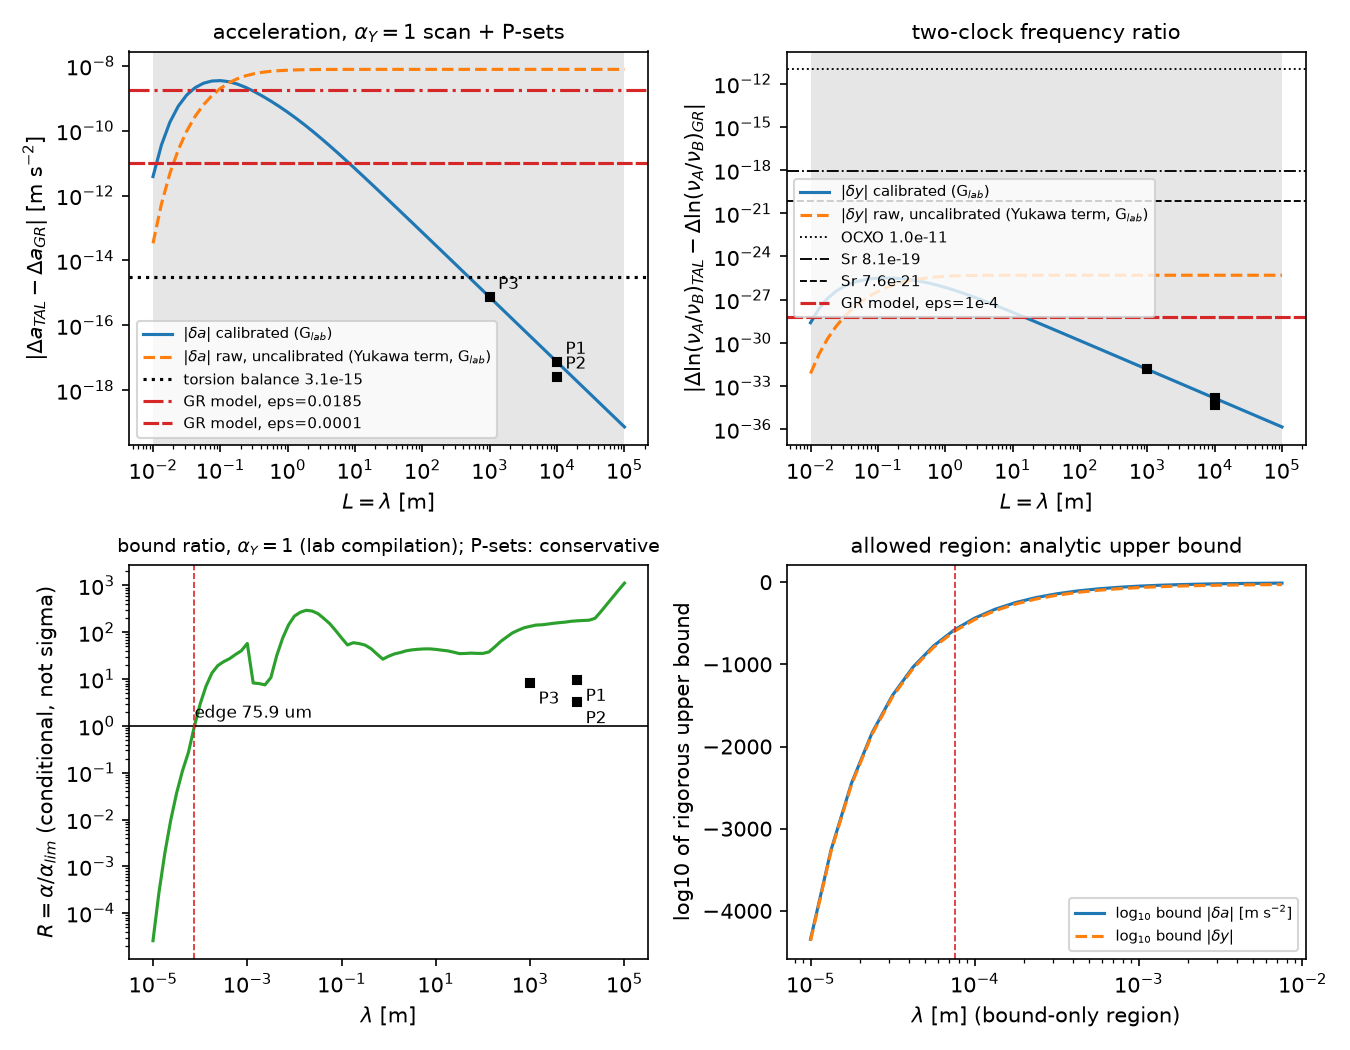
\includegraphics[width=0.9\textwidth]{../figures/fig_delta_vs_lambda.png}
\caption{Az óramodul ábrája (angol feliratokkal): $|\delta a|$ és $|\delta y|$ az $L$ függvényében $\alpha_Y=1$-re és P1--P3-ra;
az $R$ arány; valamint $10^{\V{quadLo}}\mU$ alatt az analitikus felső korlát. A szaggatott nyers görbék kalibrálatlan szemléltetések.}\label{fig:clock}
\end{figure}

\section{Yukawa-korlátok}\label{sec:bounds}
\subsection{BREN-toronylánc}\label{sec:bren}
A BREN-modul a toronyjelentések [Kasameyer 1989; Kammeraad 1990] folytatási operátorát egy forrásmodellre alkalmazza, és egy
Yukawa-tag toronyreziduumát a V28 Step~27 sík féltér-alakjával veti össze, az $\alpha=\V{brAlpha}$, $\lambda=\V{brLam}\kmu$
modellpontban. A forrásmodell szintetikus gyűrűsugarakat ($\V{nRings}$ gyűrű, $\V{nStations}$ állomás; a jelentések a darabszámokat
megadják, a sugarakat nem), modern helyettesítő DEM-et (Copernicus GLO-90, $\V{nGrid}\times\V{nGrid}$ cella, $\V{cellM}\mU$-es) és
homogén sűrűséget használ. Az eredeti állomás- és adatláncot nem rekonstruáljuk, ezért ez nem a kísérlet empirikus újraelemzése.
A megfigyelhető referenciapontja $z_0=\V{zNull}\mU$ (K90); a V28 Step~27 számai $z_0=0$-val készültek, ezeket külön tartjuk
($R=\V{RvNullTwo}$ $\rho=\V{rho2000}\kgm$ és $\V{RvNullThree}$ $\V{rho2670}\kgm$ mellett, pontosan reprodukálva).
%CAV:bren_not_empirical
%CAV:z0_separate

Változatok: A, gömbi kernel a nyers, csonkolt súlyokkal (összegük $\V{wsum}$, $\V{Rtrunc}\kmu$-es csonkolással); B, nulla összegre
normált súlyok; C, sík kernel; D, mint A, a newtoni torzítás lineáris illesztésével. Az A változat csonkolásérzékenysége operátortulajdonság,
nem terepjel, és az A és B közötti eltérés nem bizonytalansági sáv. A csúcsponton ($\V{zBN}\mU$, $\rho=\V{rho2200}\kgm$) a sík reziduum
$\V{topFlat}\uGal$; A $\V{topA}\uGal$-t, B $\V{topB}\uGal$-t ad; A tisztán operátor-része $\V{topOpA}\uGal$; a minden változatban közös terepi rész $\V{topTerr}\uGal$
(a sík érték $\V{topTerrPct}\pct$-a). Független ellenőrzésként a newtoni tereptorzítás (közvetlen mínusz folytatott)
$\V{nbias}\uGal$, szemben a jelentés $\V{nbiasRep}\pm\V{nbiasRepSig}\uGal$ értékével, illetve $\V{zKEN}\mU$-en $\rho=\V{rho1800}\kgm$ mellett $\V{nbiasKEN}\uGal$ a K89 kb.\ $\V{nbiasKENrep}\uGal$ értékével szemben (hangolás nélkül).
%CAV:A_truncation_not_terrain

Két feltételes egypontos összevetést használunk. B89: a K89 reziduum, $\V{kRes}\pm\V{kSig}\uGal$ a $\V{zKEN}\mU$-es csúcson,
konzervatív előjellel és $k=\V{kSigma}$-vel $\V{edgeBEN}\uGal$-os határt ad. B90: a K90 1.~ábrájának digitalizált method-1 csúcspontja,
$+\V{yBN}\pm\V{sBN}\uGal$ $\V{zBN}\mU$-nél (toronymagasság $\V{hKN}\mU$), $\V{edgeBN}\uGal$-t ad. Mindkettő csak egyetlen előre
kiválasztott pont varianciáját használja; a más magasságokkal vett nem diagonális kovariancia nem lép be egy egypontos marginális
tesztbe, amit a \file{check_single_point_marginal.py} megerősít ($\V{nCov}$ kovarianciaszerkezetből $\V{nCovSame}$ nem változtatja a
határt). A K90 korrelált $\chi^2$-elemzését nem reprodukáljuk. A \ref{tab:brenR}.~táblázat a $\lambda=\V{brLam}\kmu$-es arányokat adja,
soronként sűrűséggel, magassággal és konstrukcióval.
%CAV:single_point_conditional
%CAV:K90_not_reproduced
\begin{table}[htbp]\centering\small\setlength{\tabcolsep}{5pt}
\caption{BREN: $R=\alpha/\alpha_{\rm lim}$ $\lambda=\V{brLam}\kmu$, $z_0=\V{zNull}\mU$, $k=\V{kSigma}$ mellett. B89: K89 csúcspont,
$\V{zKEN}\mU$; B90: K90 1.~ábra csúcspontja, $\V{zBN}\mU$ (feltételes egypontos összevetések; nem $\sigma$).}\label{tab:brenR}
\begin{tabular}{llccccc}\toprule
$\rho$ (\kgm) & korlát & $R$ sík & $R$ A & $R$ B & $R$ C & $R$ D\\\midrule
\tabinput ../generated/tab_brenR.tex
\bottomrule\end{tabular}\end{table}

A DEM-előkészítés helyi ekvirektanguláris leképezést használ; a kelet--nyugati metrika az északi és déli szélen legfeljebb
$\V{metricPct}\pct$-kal változik. Ez deklarált korlát; nincs korrigálva, és nem jelent automatikusan ekkora reziduális hibát.
%CAV:dem_metric

\begin{figure}[tbp]\centering
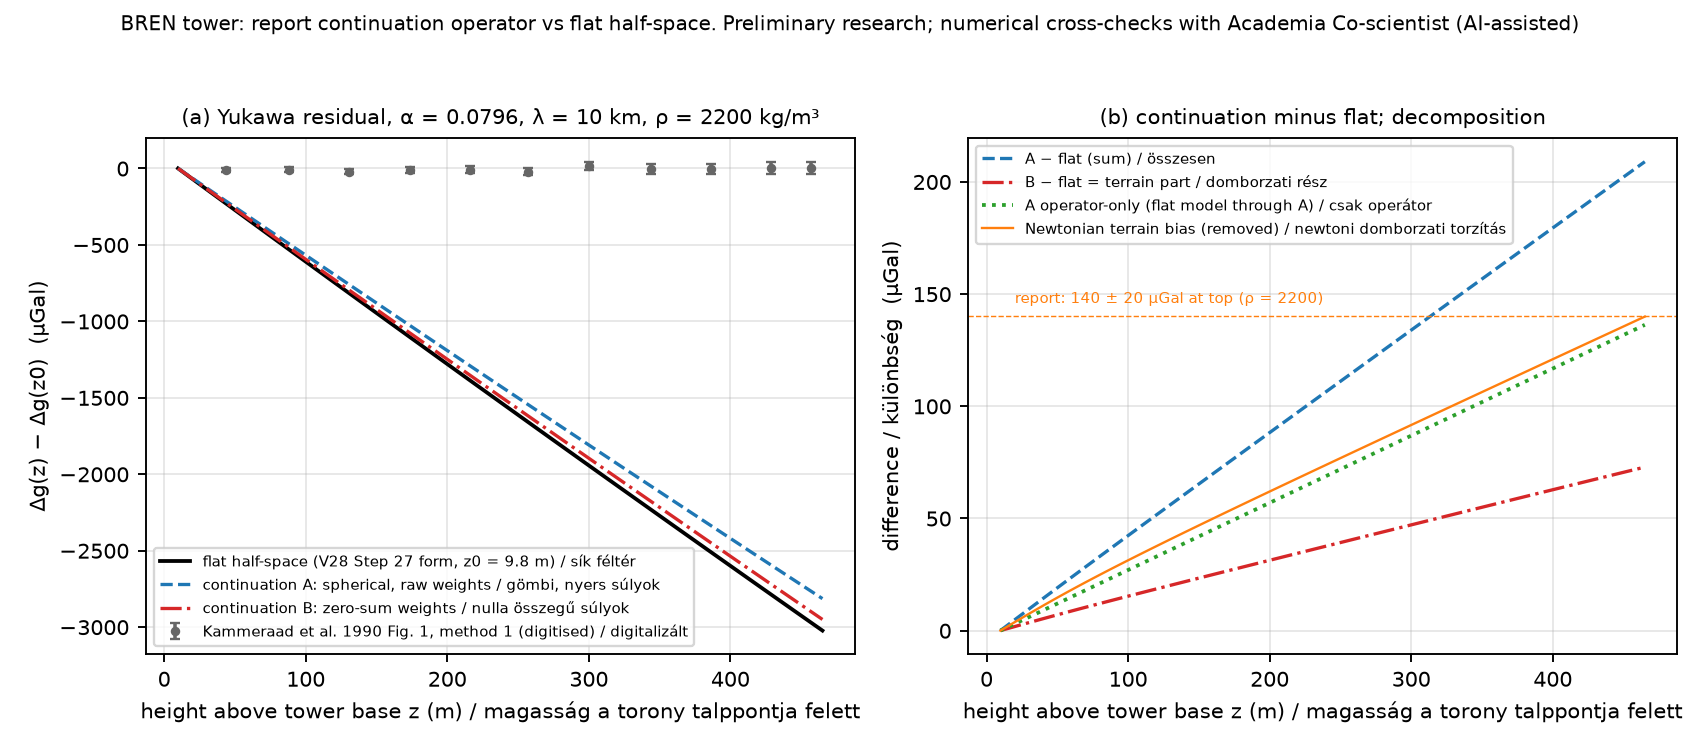
\includegraphics[width=\textwidth]{../figures/fig_residual_curve.png}
\caption{A BREN-modul ábrája: (a) a Yukawa-reziduum a magasság függvényében a sík féltérre és az A, B változatra, a digitalizált
K90-pontokkal; (b) a folytatás mínusz a sík érték, felbontva.}\label{fig:bren}
\end{figure}

\subsection{Szub-centiméteres lánc}\label{sec:subcm}
A szub-cm-modul az $\alpha=\V{scAlpha}$ értéket közölt rövid hatótávú korlátokkal ($\V{CL}\pct$ CL) veti össze, amelyeket
Adelberger et al.\ 2003 és Lee et al.\ 2020 ábráiból vektorosan digitalizáltunk, valamint a Lee 2020 disszertáció 11.4.~táblázatával
($\V{nThesis}$ sor). Az átmeneti sáv határai:
$\V{eHust}\um$ (HUST 2020 $|\alpha|$-görbe, leolvasási intervallum $\V{loHust}$--$\V{hiHust}\um$),
$\V{eEW}\um$ (Eöt-Wash 2020 $|\alpha|$-görbe, $\V{loEW}$--$\V{hiEW}\um$),
$\V{eAbs}\um$ (disszertáció, $|\alpha_{95}|$, $\V{loAbs}$--$\V{hiAbs}\um$) és
$\V{ePlus}\um$ (disszertáció, $+\alpha_{95}$, $\V{loPlus}$--$\V{hiPlus}\um$).
A sáv nem csupán HUST-előjelkérdés. $\V{eHust}$-tól kb.\ $\V{eEW}\um$-ig $\alpha$ csak akkor kizárt, ha a HUST 2020/2016
$|\alpha|$-görbéit $\alpha>0$-ra alkalmazzuk. Kb.\ $\V{eEW}$-tól $\V{ePlus}\um$-ig a két Eöt-Wash 2020 konstrukció HUST-görbe nélkül
is eltér: a disszertáció a $\pm\alpha_{95}$-öt a $\Delta\chi^2=\V{dchi}$ felületből, a $|\alpha_{95}|$-öt normális integrálból
definiálja; a $\V{rowLam}\um$-es sorban $+\alpha_{95}=\V{rowPlus}>\alpha>|\alpha_{95}|=\V{rowAbs}$. A korlátokat a közölt formában
használjuk. A leolvasási intervallumok a digitalizálásból származnak, nem fizikai bizonytalanságok.
A $\lambda<\V{eHust}\um$ tartományban az $\alpha=q$ értéket a vizsgált korlátok nem zárják ki; az újabb korlátok keresése nem volt
kimerítő.
%CAV:band_not_hust_only
%CAV:digitization_not_physical
%CAV:not_exhaustive
\begin{table}[htbp]\centering\small
\caption{Szub-cm: $R=\alpha/\alpha_{\rm lim}$ kiválasztott $\lambda$ értékeknél (feltételes, nem $\sigma$).}\label{tab:subcmR}
\begin{tabular}{lcc}\toprule
$\lambda$ (\textmu m) & $R$, disszertáció $+\alpha_{95}$ & $R$, rajzolt $|\alpha|$-burkoló\\\midrule
\tabinput ../generated/tab_subcmR.tex
\bottomrule\end{tabular}\end{table}

\begin{figure}[tbp]\centering
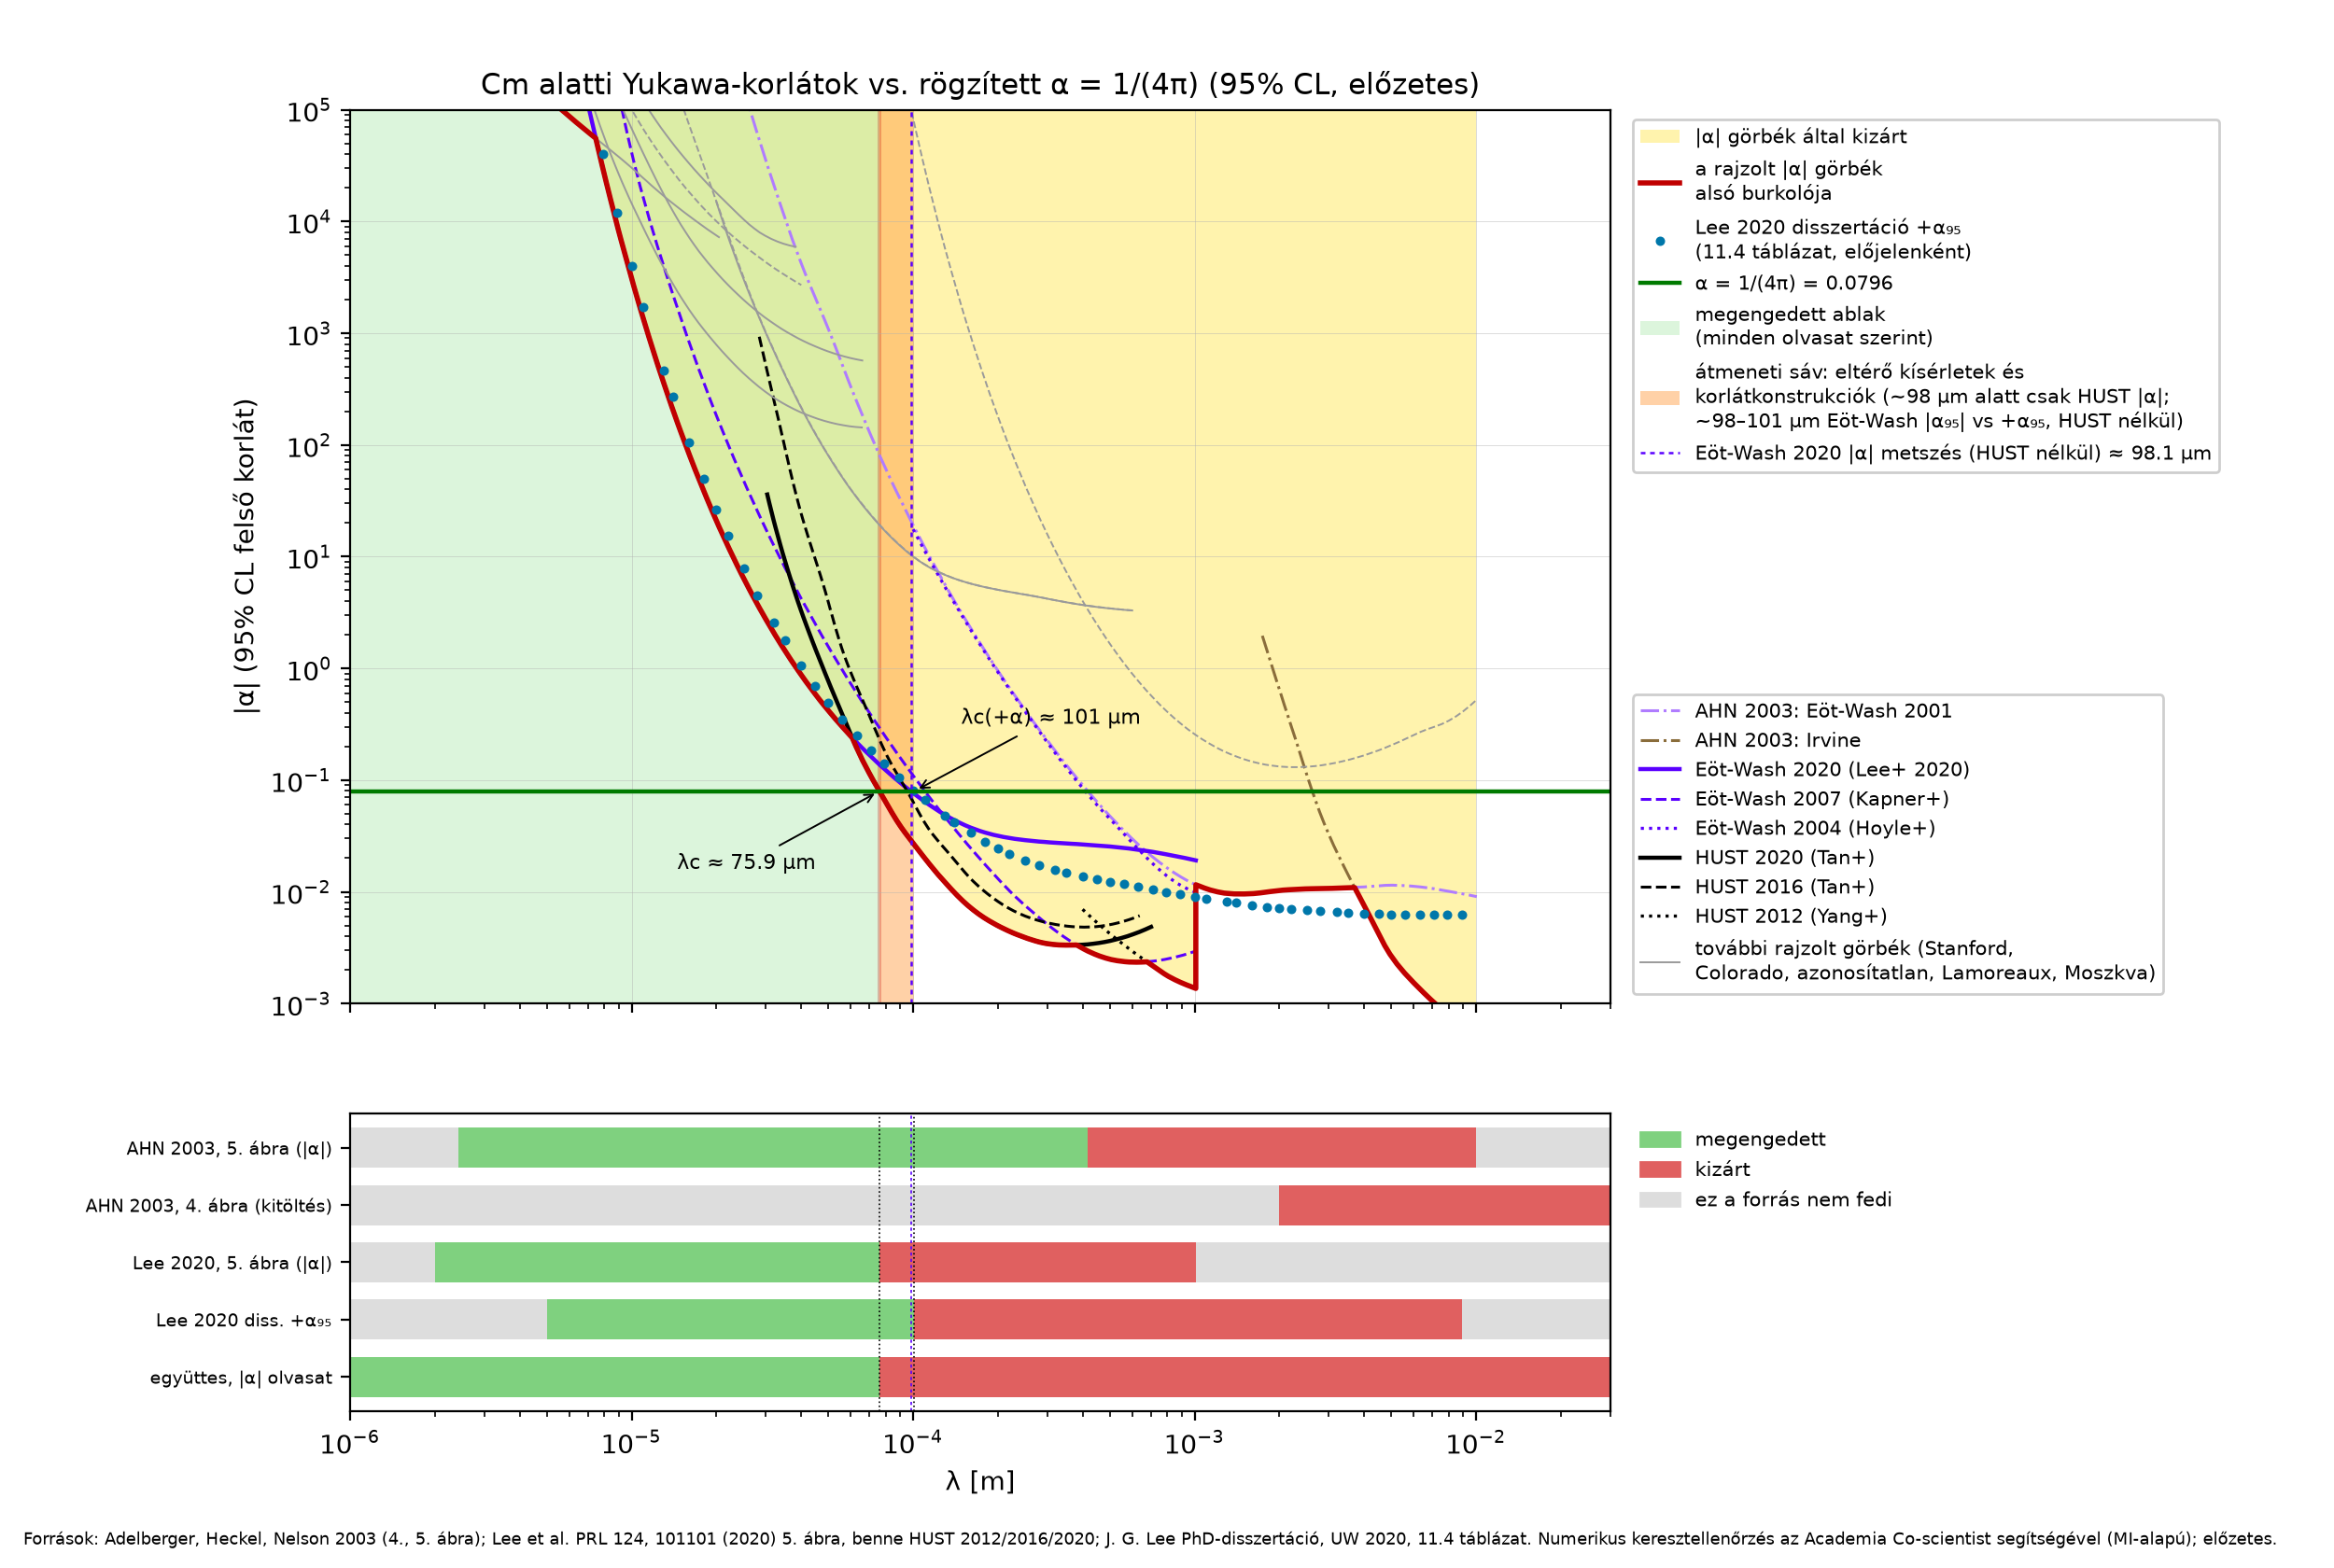
\includegraphics[width=\textwidth]{../figures/subcm_window_hu.png}
\caption{A szub-cm-modul ábrája: a rajzolt $|\alpha|$-korlátok, a disszertáció $+\alpha_{95}$-pontjai és az $\alpha=1/(4\pi)$ érték,
az átmeneti sávval.}\label{fig:subcm}
\end{figure}

\subsection{Arányok P1--P3-ra}\label{sec:ratio}
Az $R=\alpha/\alpha_{\rm lim}$ egy korláthoz viszonyított feltételes arány, nem szignifikancia: $R$ nem a szórások száma, és a
korlátok különböző szinteken értendők ($k=\V{kSigma}$ vagy $\V{CL}\pct$ CL a laboratóriumi és a BREN egypontos határokra,
$1\sigma$ az idézett K90-határra). A \ref{tab:bounds}.~táblázat a laboratóriumi kompilációt (Adelberger et al.\ 2003 4.~ábra
$\V{eFigFour}\mmu$ fölött, a szub-cm burkolóval) és a $\rho=\V{rho2000}\kgm$-es BREN B89 határokat (A--C változat) kombinálja.
P3-ra a K90 jelentés $\V{aLimKN}$ határa $\V{LP3}\kmu$-nél $R=\V{RKN}$-et ad; a projekt B90 egypontos értéke, $\V{aLimBNsp}$
($R=\V{RBNsp}$), más konstrukció, csak kontextus, és nem lép be a konzervatív arányba.
Az U feltevés mellett a vöröseltolódás-tesztek [Takamoto 2020; Grotti 2018] és a MICROSCOPE-teszt [Touboul 2022] nem korlátozza az ágat.
%CAV:R_not_sigma
\begin{table}[htbp]\centering\small\setlength{\tabcolsep}{3.5pt}
\caption{Korlátarányok (feltételes, nem $\sigma$) és kategóriák.}\label{tab:bounds}
\begin{tabular}{lcccccc}\toprule
készlet & $\alpha_{\rm lim}$ lab. & $R$ lab. & $\alpha_{\rm lim}$ BREN (A, B, C) & $R$ BREN & $R$ konzervatív & kategória\\\midrule
\tabinput ../generated/tab_bounds.tex
\bottomrule\end{tabular}\end{table}

\section{Következtetés}\label{sec:concl}
\begin{itemize}
\item A rögzített ág (P1, P2, P3) a (b) kategóriába tartozik: $\delta y\ne0$ és $\delta a\ne0$, de az erőt a vizsgált korlátok
kizárják, a legkisebb arányok $R=\V{RConsP1}$, $\V{RConsP2}$, $\V{RConsP3}$ (BREN, a vizsgált modelleken belül, feltételesen).
\item $\alpha_Y=1$ esetén a $\lambda<\V{lamEdge}\um$ tartományt a vizsgált korlátok nem zárják ki, kategóriája (\V{catRem}):
itt $\log_{10}|\delta a/(\mathrm{m\,s^{-2}})|\le\V{logDaEdge}$ és $\log_{10}|\delta y|\le\V{logDyEdge}$. A legtágabb olvasatban,
$\V{ePlus}\um$-ig, a korlát $\log_{10}|\delta a/(\mathrm{m\,s^{-2}})|\le\V{logDaPlus}$ és $\log_{10}|\delta y|\le\V{logDyPlus}$,
kategória (\V{catBand}). Ez a következtetés a deklarált geometriára vonatkozik, amelynek legközelebbi tömege $\V{dmin}\mU$-re
van az óráktól.
\item Ebben az elrendezésben ennek az ágnak nincs (d) kategóriájú tesztje. Egy rövid hatótávú erőteszt vizsgálhatná az $\alpha_Y=1$
esetet: $\lambda=\V{lamFifty}\um$-nél a rajzolt burkoló $R=\V{Rfifty}$-et ad, így egy ott kb.\ $\V{ImpFifty}$-szor érzékenyebb
torziós inga érné el az $R=1$-et. Ez erőkísérlet, nem órakísérlet.
\end{itemize}
Az itt közölt ellenőrzések technikai jellegűek (szkriptelt reprodukció, numerikus összevetés, negatív kontrollok); egy sikeres
ellenőrzés nem az ág empirikus megerősítése. Az ellenőrzések módja: numerikus keresztellenőrzés az Academia Co-scientist segítségével (MI-alapú).
%CAV:pass_technical

\appendix
\section{A BREN-operátor}\label{app:bren}
A K89 7.~egyenlete (= K90 2.~egyenlete) szerinti operátor a gömbi Poisson-kifejtés $z/a$ rendig:
\begin{equation}
\Delta g(z)=\frac{z(1-2z/a)}{2\pi}\int\!\!\int\frac{\Delta g(0,r',\varphi)\,r'\,dr'\,d\varphi}{\big[r'^2+z^2(1-z/a)\big]^{3/2}},
\qquad a=\V{aEarth}\kmu,
\end{equation}
gyűrűkre diszkretizálva; az $i$-edik gyűrű ($r_1,r_2$ sugarak) a szektorállomásai átlagát viszi, szorozva
$K_i(z)=z(1-2z/a)\big[(r_1^2+b^2)^{-1/2}-(r_2^2+b^2)^{-1/2}\big]$-vel, ahol $b^2=z^2(1-z/a)$, $\V{Rtrunc}\kmu$-es csonkolással.
Ha $T$ a közvetlen toronyérték és $P$ a folytatott érték, $B_X(z)=[T_X(z)-T_X(z_0)]-[P_X(z)-P_X(z_0)]$ a newtoni ($X=N$) és a
Yukawa- ($X=Y$) részre, a Yukawa-reziduum $\Delta g=G_\infty\alpha\rho\,(B_Y-B_N)$; sík határesetben a Step~27 alakot adja vissza.
A torony helye $\V{towerLat}\degu$\,É, $\V{towerLon}\degu$\,Ny; $\V{nPrisms}$ előjeles terepprizma.
Konvergencia a csúcson ($\rho=\V{rho2200}\kgm$, az alapon kívül $\V{nConv}$ konfiguráció): a B változat legfeljebb
$\V{convBmax}\uGal$-lal változik; az A változat $R_{\rm trunc}=\V{rtSixty}\kmu$-nél $\V{convAsixty}\uGal$, $\V{rtFour}\kmu$-nél
$\V{convAfour}\uGal$, ahogy a csonkolási tagtól várható; a newtoni torzítás $\V{convNmin}$--$\V{convNmax}\uGal$ között van, és a
Yukawa-reziduumban kiesik. A \ref{tab:brenLam}.~táblázat $\alpha_{\rm lim}$-et mutatja $\lambda$ függvényében (B89, $\rho=\V{rho2000}\kgm$).
\begin{table}[htbp]\centering\small
\caption{BREN: $\alpha_{\rm lim}$ a $\lambda$ függvényében (B89, $\rho=\V{rho2000}\kgm$).}\label{tab:brenLam}
\begin{tabular}{lccc}\toprule
$\lambda$ (km) & sík & A & B\\\midrule
\tabinput ../generated/tab_brenLam.tex
\bottomrule\end{tabular}\end{table}

\section{Digitalizálás és korlátkonstrukciók}\label{app:digit}
A szub-cm görbéket a közölt ábrák vektoros tartalmából digitalizáltuk (vonalútvonalak, tengelykalibráció az összes osztásjelre
illesztve), és raszteres leolvasással ellenőriztük; a disszertáció táblázatát a szövegrétegből olvastuk ki. A digitalizált
értékek a modulban befagyasztva, SHA-256 összegekkel szerepelnek, és ezek az alapfutás bemenetei. A konstrukciók eltérnek:
a rajzolt $|\alpha|$-görbék $|\alpha|$-ra vonatkozó korlátok; a disszertáció $\pm\alpha_{95}$ értékei a $\Delta\chi^2=\V{dchi}$
felületből jönnek; a $|\alpha_{95}|$ a $-|\alpha_{95}|$ és $+|\alpha_{95}|$ közötti normális integrálból. A régebbi AHN 2003
5.~ábra burkolója egyedül $\V{eAHN}\um$-re tenné a határt; a HUST 2016 görbe $\V{eHustSix}\um$-nél metsz; a HUST-mentes rés
$\V{eGap}\um$ széles. A BREN-nél a B89 a K89-ben közölt értéket használja $k=\V{kSigma}$-vel, a B90 pedig a K90 1.~ábrájáról
digitalizált pontot; magát a K90-határt ($1\sigma$, globális, több magasságot használó korrelált $\chi^2$) idézzük, nem számoljuk újra.
%CAV:constructions_differ

\section{Nem univerzális kiegészítés (a rögzített ágon kívül)}\label{app:addon}
Ez a függelék a rögzített ágon kívüli szemléltetés, és nem lép be a döntésbe. Ha az órafrekvenciának anomális érzékenysége volna,
$\nu\propto e^{-(1+k_c)\phi}$, akkor $\delta y_{\rm extra}=-k_c\,\Delta(\phi_A-\phi_B)$, ahol $\phi$ normálása $G_\infty$-nel történik
(az r4 modulváltozatban javítva). A \ref{tab:addon}.~táblázat a $k_c=1$-hez tartozó $\delta y_{\rm extra}$ értéket és az Sr
differenciális szinten $S=\V{Sthr}$-höz szükséges $k_c$-t adja. A $\xi_{\rm Ti}=\V{xiTi}$, $\xi_{\rm Pt}=\V{xiPt}$ Coulomb-energia-hányadokkal
és a MICROSCOPE $|\eta|<\V{etaNF}$ értékkel képzett hosszú hatótávú proxy $|k_c|\lesssim\V{kcMax}$-et ad; ezt a proxyt nem visszük át
az $L=\V{LP3}$--$\V{LP1}\kmu$ tartományra.
%CAV:addon_outside
\begin{table}[htbp]\centering\small
\caption{Nem univerzális kiegészítés (csak szemléltetés).}\label{tab:addon}
\begin{tabular}{lccc}\toprule
készlet & $G_\infty/G_{\rm lab}$ & $\delta y_{\rm extra}$ ($k_c=1$) & $k_c$ az $S=\V{Sthr}$-hez\\\midrule
\tabinput ../generated/tab_addon.tex
\bottomrule\end{tabular}\end{table}

\section*{Adatok és kód elérhetősége}\label{sec:avail}
A három modularchívum változatlanul, SHA-256 összegekkel szerepel a publikációs készletben:
\begin{itemize}\setlength{\itemsep}{0pt}
\item \file{tal_branch_clock_accel_test_r4.zip} (óra és gyorsulás, fő elemzés);
\item \file{bren_continuation_zenodo_r4.zip} (BREN-torony folytatása);
\item \file{subcm_yukawa_window_zenodo_r4.zip} (szub-centiméteres Yukawa-ablak).
\end{itemize}
A közlemény forrásai, az állítás--forrás táblázat és az ellenőrző szkriptje az \file{article/} mappában van. A TAL-mű koncepció-DOI-ja:
\doi{10.5281/zenodo.22983681}; kapcsolódó rekordok: V20 \doi{10.5281/zenodo.23540741}, V26 \doi{10.5281/zenodo.23727585},
V28 \doi{10.5281/zenodo.23814053}. Licenc: CC BY-NC 4.0 Nemzetközi; harmadik fél dokumentumaira és adataira a saját feltételeik vonatkoznak.

\section*{Hivatkozások}
\footnotesize
\begin{itemize}\setlength{\itemsep}{0pt}
\item E. G. Adelberger, B. R. Heckel, A. E. Nelson, Annu.\ Rev.\ Nucl.\ Part.\ Sci.\ 53, 77 (2003), arXiv:hep-ph/0307284.
\item J. G. Lee, E. G. Adelberger, T. S. Cook, S. M. Fleischer, B. R. Heckel, Phys.\ Rev.\ Lett.\ 124, 101101 (2020), arXiv:2002.11761.
\item J. G. Lee, PhD-disszertáció, University of Washington (2020), \url{https://hdl.handle.net/1773/45542}, 11.4. táblázat.
\item W.-H. Tan et al., Phys.\ Rev.\ Lett.\ 124, 051301 (2020); W.-H. Tan et al., Phys.\ Rev.\ Lett.\ 116, 131101 (2016).
\item D. J. Kapner et al., Phys.\ Rev.\ Lett.\ 98, 021101 (2007); C. D. Hoyle et al., Phys.\ Rev.\ D 70, 042004 (2004).
\item P. Kasameyer et al., UCRL-101001 (1989), OSTI 6190822 [K89]; J. Kammeraad et al., UCRL-JC-103562 (1990), OSTI 6993119 [K90].
\item T. Bothwell et al., Nature 602, 420 (2022); M. Aeppli et al., Phys.\ Rev.\ Lett.\ 133, 023401 (2024).
\item S. Schlamminger et al., Phys.\ Rev.\ Lett.\ 100, 041101 (2008); P. Touboul et al., Phys.\ Rev.\ Lett.\ 129, 121102 (2022).
\item M. Takamoto et al., Nat.\ Photon.\ 14, 411 (2020); J. Grotti et al., Nat.\ Phys.\ 14, 437 (2018).
\item Oscilloquartz 8662/8663 specifikáció (2003. március); CODATA 2018 ajánlott értékek; Copernicus GLO-90 DEM.
\end{itemize}
\end{document}
